
\documentclass{report}
\usepackage[utf8]{inputenc}
\usepackage{graphicx}
\usepackage{booktabs}
\usepackage{geometry}
\usepackage{hyperref}
\usepackage{multirow}
\usepackage{longtable}
\usepackage{float}
\geometry{a4paper, margin=1in}

\title{Comprehensive Analysis of Dengue Epidemic Forecasting across Brazilian Regions}
\author{Antigravity Analysis Engine}
\date{\today}

\begin{document}

\maketitle

\chapter{Data Overview and Scaling Analysis}

\section{Dataset Composition}
The analysis integrates state-level and city-level data from 2010 to 2024. Table \ref{tab:dataset_stats} summarizes the training volume for each state.

\begin{center}
\begingroup
\renewcommand{\arraystretch}{1.1}
\begin{longtable}{lrrr}
\caption{Dataset Statistics by State} \label{tab:dataset_stats} \\
\toprule
State & Cities & Total Obs. & Total Pop. \\
\midrule
\endfirsthead
\caption[]{Dataset Statistics by State} \\
\toprule
State & Cities & Total Obs. & Total Pop. \\
\midrule
\endhead
\midrule
\multicolumn{4}{r}{Continued on next page} \\
\midrule
\endfoot
\bottomrule
\endlastfoot
AC & 20 & 144 & 811003.000000 \\
AL & 68 & 302 & 2840500.000000 \\
AM & 38 & 227 & 3512889.000000 \\
AP & 11 & 72 & 741209.000000 \\
BA & 368 & 1706 & 14017230.000000 \\
CE & 169 & 1125 & 8764130.000000 \\
DF & 1 & 14 & 2923369.000000 \\
ES & 77 & 545 & 3968431.000000 \\
GO & 224 & 1500 & 6882117.000000 \\
MA & 79 & 253 & 4607990.000000 \\
MG & 679 & 3396 & 19763429.000000 \\
MS & 79 & 647 & 2833742.000000 \\
MT & 122 & 795 & 3707334.000000 \\
PA & 109 & 558 & 7785797.000000 \\
PB & 121 & 466 & 3404005.000000 \\
PE & 158 & 918 & 8641573.000000 \\
PI & 65 & 206 & 2296908.000000 \\
PR & 341 & 2004 & 11132125.000000 \\
RJ & 92 & 678 & 16615526.000000 \\
RN & 124 & 560 & 3070185.000000 \\
RO & 47 & 306 & 1583409.000000 \\
RR & 13 & 87 & 604047.000000 \\
RS & 150 & 339 & 8516859.000000 \\
SC & 116 & 333 & 6207938.000000 \\
SE & 28 & 138 & 1699031.000000 \\
SP & 623 & 4460 & 45915564.000000 \\
TO & 63 & 304 & 1272148.000000 \\
\end{longtable}

\endgroup
\endcenter

\section{Scaling and Power Law Dynamics}
A fundamental component of our methodology is the assumption that epidemic sizes follow a Power Law distribution. Figure \ref{fig:pl_dist} shows the distribution of the scaling parameter $\alpha$ identified across thousands of city outbreaks.

\begin{figure}[H]
    \centering
    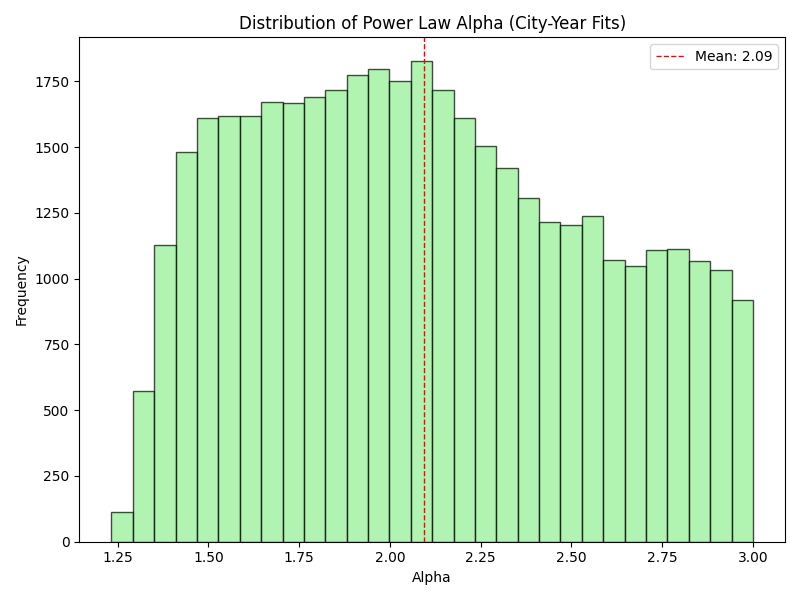
\includegraphics[width=0.7\textwidth]{report_assets/pl_alpha_dist.png}
    \caption{Distribution of the Power Law $\alpha$ parameter for municipality outbreaks.}
    \label{fig:pl_dist}
\end{figure}

The mean observed $\alpha \approx 2.36$ suggests a robust structural scale-invariance in Dengue propagation.

\chapter{Model Performance and Regional Variation}

\section{National Predictive Accuracy}
We utilize Random Forest Regressors with log-transformed targets (\textit{total\_cases}) to handle the order-of-magnitude variations in outbreak sizes.

\begin{figure}[H]
    \centering
    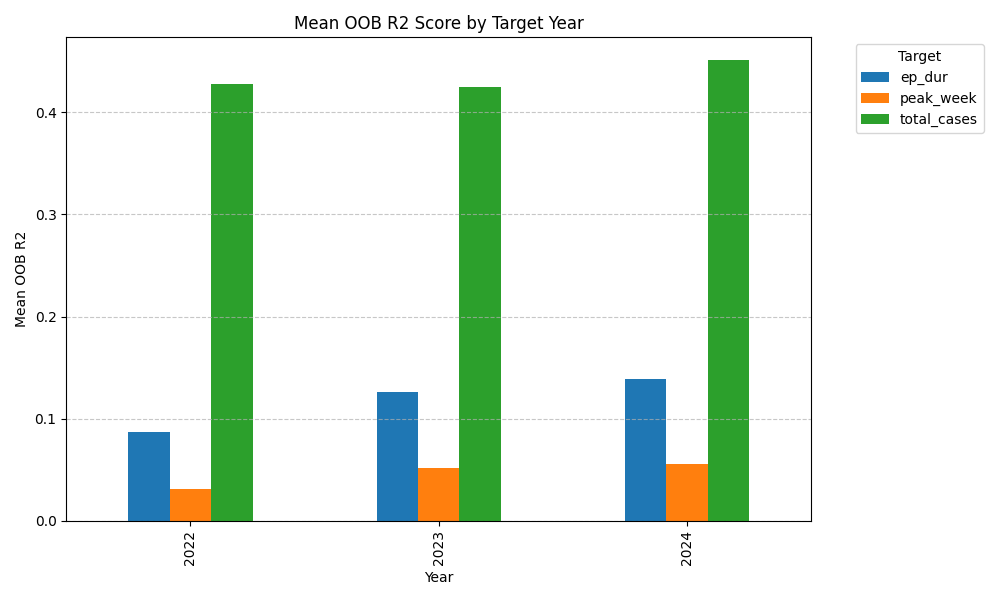
\includegraphics[width=0.9\textwidth]{report_assets/performance_by_year.png}
    \caption{National average performance (OOB R2) trends.}
\end{figure}

\section{Regional Heterogeneity}
Regional differences in climate, urban density, and reporting accuracy significantly influence model skill. Figure \ref{fig:reg_perf} highlights performance variation across Brazil's five macro-regions.

\begin{figure}[H]
    \centering
    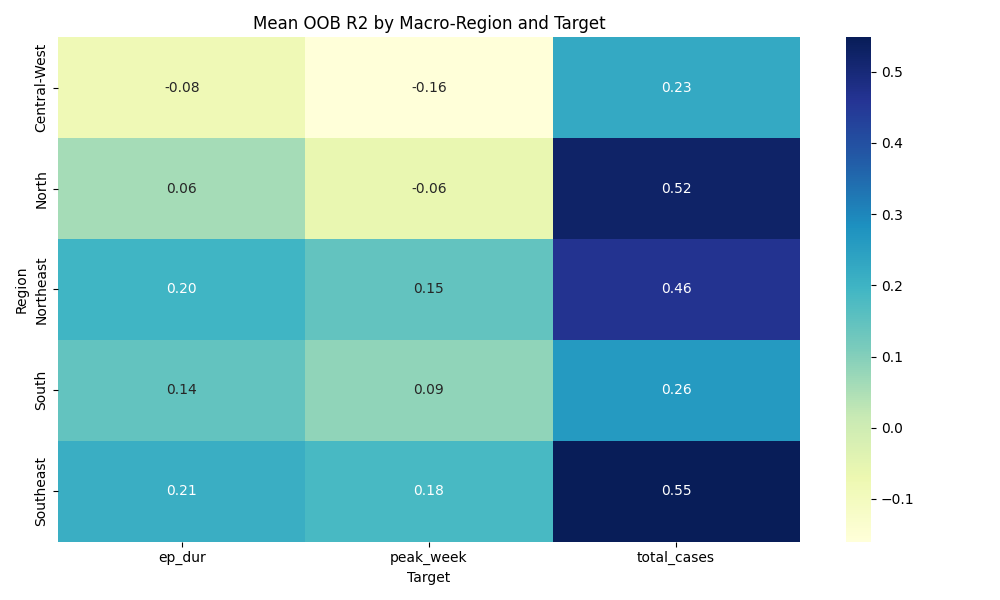
\includegraphics[width=0.8\textwidth]{report_assets/regional_performance.png}
    \caption{Mean OOB R2 by Macro-Region. North and Northeast regions show distinct patterns compared to the Southeast.}
    \label{fig:reg_perf}
\end{figure}

\section{State-Level Performance Breakdown}
Detailed metrics for each state and target years are provided for exhaustive reference.

\begin{center}
\begingroup
\tiny
\begin{longtable}{llllrrr}
\caption{Detailed State Metrics (2022-2024)} \\
\toprule
 &  &  & Region & MAE & RMSE & OOB\_R2 \\
Year & State & Target &  &  &  &  \\
\midrule
\endfirsthead
\caption[]{Detailed State Metrics (2022-2024)} \\
\toprule
 &  &  & Region & MAE & RMSE & OOB\_R2 \\
Year & State & Target &  &  &  &  \\
\midrule
\endhead
\midrule
\multicolumn{7}{r}{Continued on next page} \\
\midrule
\endfoot
\bottomrule
\endlastfoot
\multirow[t]{81}{*}{2022} & \multirow[t]{3}{*}{RO} & total\_cases & North & 325.378983 & 638.578411 & 0.344968 \\
 &  & ep\_dur & North & 10.475958 & 12.641191 & 0.027167 \\
 &  & peak\_week & North & 5.891524 & 7.387133 & -0.051143 \\
\cline{2-7}
 & \multirow[t]{3}{*}{AC} & total\_cases & North & 925.851397 & 2139.882758 & 0.663701 \\
 &  & ep\_dur & North & 10.250667 & 12.430286 & -0.058569 \\
 &  & peak\_week & North & 5.398700 & 6.813211 & -0.051293 \\
\cline{2-7}
 & \multirow[t]{3}{*}{AM} & total\_cases & North & 453.909437 & 902.536954 & 0.428859 \\
 &  & ep\_dur & North & 9.755690 & 11.942594 & -0.006342 \\
 &  & peak\_week & North & 6.510892 & 8.065748 & 0.058174 \\
\cline{2-7}
 & \multirow[t]{3}{*}{RR} & total\_cases & North & 166.163402 & 353.527859 & 0.609734 \\
 &  & ep\_dur & North & 8.995309 & 10.654837 & 0.018497 \\
 &  & peak\_week & North & 5.075374 & 5.952405 & -0.237164 \\
\cline{2-7}
 & \multirow[t]{3}{*}{PA} & total\_cases & North & 315.272296 & 663.623560 & 0.375528 \\
 &  & ep\_dur & North & 8.695886 & 10.475612 & 0.034659 \\
 &  & peak\_week & North & 4.655746 & 6.175117 & -0.037305 \\
\cline{2-7}
 & \multirow[t]{3}{*}{AP} & total\_cases & North & 861.542965 & 1903.667477 & 0.516009 \\
 &  & ep\_dur & North & 9.214815 & 11.249707 & 0.213630 \\
 &  & peak\_week & North & 7.447090 & 8.735796 & -0.029359 \\
\cline{2-7}
 & \multirow[t]{3}{*}{TO} & total\_cases & North & 468.725295 & 1674.609599 & 0.706169 \\
 &  & ep\_dur & North & 7.180118 & 8.701952 & 0.108934 \\
 &  & peak\_week & North & 3.782875 & 5.316473 & -0.021521 \\
\cline{2-7}
 & \multirow[t]{3}{*}{MA} & total\_cases & Northeast & 202.706175 & 495.775966 & 0.335672 \\
 &  & ep\_dur & Northeast & 7.454872 & 9.417341 & 0.104771 \\
 &  & peak\_week & Northeast & 3.683200 & 4.853353 & 0.055445 \\
\cline{2-7}
 & \multirow[t]{3}{*}{PI} & total\_cases & Northeast & 420.586355 & 1637.325862 & 0.719920 \\
 &  & ep\_dur & Northeast & 7.945800 & 9.801783 & 0.161629 \\
 &  & peak\_week & Northeast & 4.243276 & 5.461066 & -0.005327 \\
\cline{2-7}
 & \multirow[t]{3}{*}{CE} & total\_cases & Northeast & 433.529103 & 1875.577237 & 0.418670 \\
 &  & ep\_dur & Northeast & 8.324841 & 10.003335 & 0.027406 \\
 &  & peak\_week & Northeast & 4.549238 & 5.458474 & 0.010549 \\
\cline{2-7}
 & \multirow[t]{3}{*}{RN} & total\_cases & Northeast & 344.847846 & 1424.815497 & 0.578098 \\
 &  & ep\_dur & Northeast & 9.267761 & 11.286522 & 0.238766 \\
 &  & peak\_week & Northeast & 5.236729 & 6.326322 & 0.245122 \\
\cline{2-7}
 & \multirow[t]{3}{*}{PB} & total\_cases & Northeast & 270.722174 & 971.687234 & 0.432482 \\
 &  & ep\_dur & Northeast & 10.050829 & 11.987025 & 0.185762 \\
 &  & peak\_week & Northeast & 4.887454 & 6.107715 & 0.102206 \\
\cline{2-7}
 & \multirow[t]{3}{*}{PE} & total\_cases & Northeast & 370.658853 & 938.618720 & 0.484534 \\
 &  & ep\_dur & Northeast & 9.662364 & 11.704810 & 0.378097 \\
 &  & peak\_week & Northeast & 4.668150 & 5.863090 & 0.520925 \\
\cline{2-7}
 & \multirow[t]{3}{*}{AL} & total\_cases & Northeast & 469.817749 & 1425.560133 & 0.533854 \\
 &  & ep\_dur & Northeast & 8.393875 & 10.196676 & 0.251046 \\
 &  & peak\_week & Northeast & 4.325088 & 5.425592 & 0.183598 \\
\cline{2-7}
 & \multirow[t]{3}{*}{SE} & total\_cases & Northeast & 424.396464 & 986.345990 & 0.390766 \\
 &  & ep\_dur & Northeast & 9.641384 & 11.727008 & 0.093719 \\
 &  & peak\_week & Northeast & 6.544143 & 8.218966 & 0.189751 \\
\cline{2-7}
 & \multirow[t]{3}{*}{BA} & total\_cases & Northeast & 521.517171 & 2110.865787 & 0.362211 \\
 &  & ep\_dur & Northeast & 8.087934 & 9.979409 & 0.229691 \\
 &  & peak\_week & Northeast & 4.277054 & 5.354088 & 0.072929 \\
\cline{2-7}
 & \multirow[t]{3}{*}{MG} & total\_cases & Southeast & 1623.190539 & 9207.619496 & 0.515284 \\
 &  & ep\_dur & Southeast & 7.324409 & 9.061016 & 0.196994 \\
 &  & peak\_week & Southeast & 3.727102 & 4.791369 & 0.068335 \\
\cline{2-7}
 & \multirow[t]{3}{*}{ES} & total\_cases & Southeast & 1669.204677 & 3566.156527 & 0.684435 \\
 &  & ep\_dur & Southeast & 8.662296 & 10.718048 & 0.284855 \\
 &  & peak\_week & Southeast & 5.119361 & 6.741328 & 0.316617 \\
\cline{2-7}
 & \multirow[t]{3}{*}{RJ} & total\_cases & Southeast & 1873.926114 & 9322.478118 & 0.476328 \\
 &  & ep\_dur & Southeast & 7.505271 & 9.189546 & 0.150577 \\
 &  & peak\_week & Southeast & 4.027199 & 4.910750 & 0.124260 \\
\cline{2-7}
 & \multirow[t]{3}{*}{SP} & total\_cases & Southeast & 2649.170990 & 28762.298747 & 0.582578 \\
 &  & ep\_dur & Southeast & 6.998510 & 8.741187 & 0.187781 \\
 &  & peak\_week & Southeast & 3.655930 & 4.641160 & 0.180613 \\
\cline{2-7}
 & \multirow[t]{3}{*}{PR} & total\_cases & South & 1249.826823 & 4248.825507 & 0.552307 \\
 &  & ep\_dur & South & 7.549541 & 9.461927 & 0.225571 \\
 &  & peak\_week & South & 3.573097 & 4.374054 & 0.173636 \\
\cline{2-7}
 & \multirow[t]{3}{*}{SC} & total\_cases & South & 3468.560130 & 12115.750356 & 0.050655 \\
 &  & ep\_dur & South & 8.508694 & 9.900695 & 0.109954 \\
 &  & peak\_week & South & 2.476898 & 3.118825 & -0.004030 \\
\cline{2-7}
 & \multirow[t]{3}{*}{RS} & total\_cases & South & 1468.530206 & 4634.398457 & 0.001152 \\
 &  & ep\_dur & South & 6.599935 & 7.944145 & -0.366885 \\
 &  & peak\_week & South & 3.795046 & 4.666855 & -0.332434 \\
\cline{2-7}
 & \multirow[t]{3}{*}{MS} & total\_cases & Central-West & 542.534783 & 1292.845658 & 0.432117 \\
 &  & ep\_dur & Central-West & 7.992186 & 9.980905 & 0.005950 \\
 &  & peak\_week & Central-West & 6.063578 & 7.425431 & 0.196628 \\
\cline{2-7}
 & \multirow[t]{3}{*}{MT} & total\_cases & Central-West & 421.322302 & 1208.698384 & 0.581896 \\
 &  & ep\_dur & Central-West & 7.616238 & 9.395467 & 0.093574 \\
 &  & peak\_week & Central-West & 4.862553 & 5.906523 & 0.031350 \\
\cline{2-7}
 & \multirow[t]{3}{*}{GO} & total\_cases & Central-West & 978.692906 & 3676.674727 & 0.651772 \\
 &  & ep\_dur & Central-West & 6.770983 & 8.421908 & 0.179108 \\
 &  & peak\_week & Central-West & 3.415758 & 4.576020 & 0.069480 \\
\cline{2-7}
 & \multirow[t]{3}{*}{DF} & total\_cases & Central-West & 98102.231228 & 155483.514860 & -0.887581 \\
 &  & ep\_dur & Central-West & 6.118333 & 7.289665 & -0.727413 \\
 &  & peak\_week & Central-West & 2.353066 & 3.924158 & -0.986366 \\
\cline{1-7} \cline{2-7}
\multirow[t]{81}{*}{2023} & \multirow[t]{3}{*}{RO} & total\_cases & North & 273.573269 & 540.323806 & 0.348467 \\
 &  & ep\_dur & North & 10.854257 & 13.087153 & 0.021310 \\
 &  & peak\_week & North & 4.743088 & 5.732432 & -0.052267 \\
\cline{2-7}
 & \multirow[t]{3}{*}{AC} & total\_cases & North & 991.817128 & 2362.638328 & 0.660257 \\
 &  & ep\_dur & North & 10.717516 & 12.958655 & -0.111772 \\
 &  & peak\_week & North & 5.550919 & 7.020246 & -0.080390 \\
\cline{2-7}
 & \multirow[t]{3}{*}{AM} & total\_cases & North & 520.105015 & 1009.239087 & 0.423209 \\
 &  & ep\_dur & North & 9.228230 & 11.398656 & -0.007801 \\
 &  & peak\_week & North & 5.951457 & 7.342933 & 0.070680 \\
\cline{2-7}
 & \multirow[t]{3}{*}{RR} & total\_cases & North & 174.042333 & 373.120383 & 0.618638 \\
 &  & ep\_dur & North & 8.324638 & 10.152814 & -0.061822 \\
 &  & peak\_week & North & 4.438005 & 5.225922 & -0.278324 \\
\cline{2-7}
 & \multirow[t]{3}{*}{PA} & total\_cases & North & 314.876609 & 661.094205 & 0.351065 \\
 &  & ep\_dur & North & 8.537478 & 10.419492 & 0.063246 \\
 &  & peak\_week & North & 4.467609 & 5.963853 & -0.045925 \\
\cline{2-7}
 & \multirow[t]{3}{*}{AP} & total\_cases & North & 971.846624 & 2030.835650 & 0.564935 \\
 &  & ep\_dur & North & 9.607500 & 11.693682 & 0.269285 \\
 &  & peak\_week & North & 6.913265 & 8.318094 & -0.004655 \\
\cline{2-7}
 & \multirow[t]{3}{*}{TO} & total\_cases & North & 309.545562 & 619.566303 & 0.706410 \\
 &  & ep\_dur & North & 7.118378 & 8.700017 & 0.166624 \\
 &  & peak\_week & North & 2.967500 & 3.757869 & -0.034934 \\
\cline{2-7}
 & \multirow[t]{3}{*}{MA} & total\_cases & Northeast & 172.378842 & 405.427584 & 0.323117 \\
 &  & ep\_dur & Northeast & 7.216803 & 9.289114 & 0.131358 \\
 &  & peak\_week & Northeast & 3.519845 & 4.510600 & 0.060677 \\
\cline{2-7}
 & \multirow[t]{3}{*}{PI} & total\_cases & Northeast & 287.076803 & 862.979306 & 0.635411 \\
 &  & ep\_dur & Northeast & 7.836458 & 9.942545 & 0.183530 \\
 &  & peak\_week & Northeast & 3.945507 & 5.068105 & -0.045979 \\
\cline{2-7}
 & \multirow[t]{3}{*}{CE} & total\_cases & Northeast & 463.299187 & 2240.413135 & 0.432012 \\
 &  & ep\_dur & Northeast & 8.105000 & 10.026070 & 0.037172 \\
 &  & peak\_week & Northeast & 4.552456 & 5.510775 & 0.019266 \\
\cline{2-7}
 & \multirow[t]{3}{*}{RN} & total\_cases & Northeast & 270.923873 & 756.384523 & 0.531434 \\
 &  & ep\_dur & Northeast & 10.507593 & 12.362390 & 0.207700 \\
 &  & peak\_week & Northeast & 6.013454 & 6.777658 & 0.217619 \\
\cline{2-7}
 & \multirow[t]{3}{*}{PB} & total\_cases & Northeast & 238.254914 & 848.558019 & 0.426053 \\
 &  & ep\_dur & Northeast & 10.640661 & 12.580950 & 0.203912 \\
 &  & peak\_week & Northeast & 4.635475 & 5.863627 & 0.066451 \\
\cline{2-7}
 & \multirow[t]{3}{*}{PE} & total\_cases & Northeast & 332.385285 & 914.143473 & 0.467895 \\
 &  & ep\_dur & Northeast & 9.708243 & 11.866194 & 0.383528 \\
 &  & peak\_week & Northeast & 4.647950 & 5.717742 & 0.468597 \\
\cline{2-7}
 & \multirow[t]{3}{*}{AL} & total\_cases & Northeast & 382.641410 & 958.822204 & 0.467433 \\
 &  & ep\_dur & Northeast & 10.022333 & 11.974813 & 0.308386 \\
 &  & peak\_week & Northeast & 4.590881 & 5.471347 & 0.195778 \\
\cline{2-7}
 & \multirow[t]{3}{*}{SE} & total\_cases & Northeast & 393.065777 & 907.101654 & 0.392947 \\
 &  & ep\_dur & Northeast & 9.540000 & 11.945309 & 0.135128 \\
 &  & peak\_week & Northeast & 7.128386 & 8.743806 & 0.246279 \\
\cline{2-7}
 & \multirow[t]{3}{*}{BA} & total\_cases & Northeast & 574.507214 & 2315.188622 & 0.355528 \\
 &  & ep\_dur & Northeast & 8.205166 & 10.172289 & 0.217783 \\
 &  & peak\_week & Northeast & 4.007884 & 5.048763 & 0.078526 \\
\cline{2-7}
 & \multirow[t]{3}{*}{MG} & total\_cases & Southeast & 1771.865418 & 9691.776861 & 0.496294 \\
 &  & ep\_dur & Southeast & 6.728968 & 8.372134 & 0.215568 \\
 &  & peak\_week & Southeast & 3.797391 & 4.928770 & 0.090015 \\
\cline{2-7}
 & \multirow[t]{3}{*}{ES} & total\_cases & Southeast & 1900.173946 & 3920.735114 & 0.653201 \\
 &  & ep\_dur & Southeast & 8.405290 & 10.438948 & 0.299121 \\
 &  & peak\_week & Southeast & 5.188738 & 6.707948 & 0.340365 \\
\cline{2-7}
 & \multirow[t]{3}{*}{RJ} & total\_cases & Southeast & 2127.719486 & 10033.926952 & 0.472273 \\
 &  & ep\_dur & Southeast & 7.126188 & 8.761826 & 0.136348 \\
 &  & peak\_week & Southeast & 3.651814 & 4.403402 & 0.145850 \\
\cline{2-7}
 & \multirow[t]{3}{*}{SP} & total\_cases & Southeast & 3160.139218 & 32632.254706 & 0.576025 \\
 &  & ep\_dur & Southeast & 6.649665 & 8.412336 & 0.185963 \\
 &  & peak\_week & Southeast & 3.149931 & 4.106911 & 0.190971 \\
\cline{2-7}
 & \multirow[t]{3}{*}{PR} & total\_cases & South & 1383.499794 & 4634.086609 & 0.497557 \\
 &  & ep\_dur & South & 6.903325 & 8.855865 & 0.203549 \\
 &  & peak\_week & South & 3.087170 & 3.871138 & 0.235970 \\
\cline{2-7}
 & \multirow[t]{3}{*}{SC} & total\_cases & South & 3470.267379 & 12265.182173 & 0.154443 \\
 &  & ep\_dur & South & 7.526753 & 9.671773 & 0.374311 \\
 &  & peak\_week & South & 2.302909 & 2.998882 & 0.138495 \\
\cline{2-7}
 & \multirow[t]{3}{*}{RS} & total\_cases & South & 1444.023000 & 4808.730360 & 0.056629 \\
 &  & ep\_dur & South & 6.409018 & 8.243836 & 0.182813 \\
 &  & peak\_week & South & 2.173638 & 2.662513 & -0.056080 \\
\cline{2-7}
 & \multirow[t]{3}{*}{MS} & total\_cases & Central-West & 603.523988 & 1430.493948 & 0.441085 \\
 &  & ep\_dur & Central-West & 7.345469 & 9.099516 & 0.120715 \\
 &  & peak\_week & Central-West & 4.374676 & 5.658380 & 0.276212 \\
\cline{2-7}
 & \multirow[t]{3}{*}{MT} & total\_cases & Central-West & 412.048124 & 1295.620256 & 0.545559 \\
 &  & ep\_dur & Central-West & 7.820634 & 9.628913 & 0.061291 \\
 &  & peak\_week & Central-West & 5.000931 & 6.163903 & 0.043234 \\
\cline{2-7}
 & \multirow[t]{3}{*}{GO} & total\_cases & Central-West & 1015.556725 & 3808.773343 & 0.647817 \\
 &  & ep\_dur & Central-West & 6.863648 & 8.661839 & 0.164515 \\
 &  & peak\_week & Central-West & 3.314502 & 4.361666 & 0.032076 \\
\cline{2-7}
 & \multirow[t]{3}{*}{DF} & total\_cases & Central-West & 104973.245580 & 173628.516566 & -0.775571 \\
 &  & ep\_dur & Central-West & 7.842222 & 8.335741 & -0.699155 \\
 &  & peak\_week & Central-West & 2.931241 & 4.513603 & -0.915710 \\
\cline{1-7} \cline{2-7}
\multirow[t]{81}{*}{2024} & \multirow[t]{3}{*}{RO} & total\_cases & North & 248.916470 & 525.377723 & 0.373868 \\
 &  & ep\_dur & North & 11.303175 & 13.487802 & -0.016435 \\
 &  & peak\_week & North & 4.810601 & 5.915931 & -0.026755 \\
\cline{2-7}
 & \multirow[t]{3}{*}{AC} & total\_cases & North & 1148.670739 & 2787.292352 & 0.662179 \\
 &  & ep\_dur & North & 11.482286 & 13.333439 & 0.035582 \\
 &  & peak\_week & North & 6.520289 & 7.863577 & -0.080644 \\
\cline{2-7}
 & \multirow[t]{3}{*}{AM} & total\_cases & North & 516.435713 & 1070.674701 & 0.410866 \\
 &  & ep\_dur & North & 9.952043 & 12.044964 & 0.022469 \\
 &  & peak\_week & North & 6.007768 & 7.364700 & 0.027592 \\
\cline{2-7}
 & \multirow[t]{3}{*}{RR} & total\_cases & North & 215.172226 & 453.552979 & 0.609649 \\
 &  & ep\_dur & North & 10.067111 & 11.480133 & 0.034137 \\
 &  & peak\_week & North & 3.853130 & 4.787645 & -0.252598 \\
\cline{2-7}
 & \multirow[t]{3}{*}{PA} & total\_cases & North & 376.012989 & 740.048370 & 0.357184 \\
 &  & ep\_dur & North & 8.493333 & 10.239016 & 0.079717 \\
 &  & peak\_week & North & 4.502999 & 5.939662 & -0.046243 \\
\cline{2-7}
 & \multirow[t]{3}{*}{AP} & total\_cases & North & 1103.488487 & 2190.765225 & 0.567351 \\
 &  & ep\_dur & North & 11.162333 & 12.947165 & 0.296205 \\
 &  & peak\_week & North & 6.756133 & 8.282233 & -0.042412 \\
\cline{2-7}
 & \multirow[t]{3}{*}{TO} & total\_cases & North & 285.000331 & 537.838095 & 0.716367 \\
 &  & ep\_dur & North & 7.098750 & 8.561710 & 0.159251 \\
 &  & peak\_week & North & 2.889529 & 3.837667 & -0.057761 \\
\cline{2-7}
 & \multirow[t]{3}{*}{MA} & total\_cases & Northeast & 165.470774 & 390.743859 & 0.371001 \\
 &  & ep\_dur & Northeast & 7.845897 & 9.529840 & 0.109055 \\
 &  & peak\_week & Northeast & 3.443925 & 4.611187 & 0.116634 \\
\cline{2-7}
 & \multirow[t]{3}{*}{PI} & total\_cases & Northeast & 286.317452 & 851.321848 & 0.665687 \\
 &  & ep\_dur & Northeast & 7.755769 & 10.057068 & 0.168910 \\
 &  & peak\_week & Northeast & 4.099077 & 5.317168 & -0.070745 \\
\cline{2-7}
 & \multirow[t]{3}{*}{CE} & total\_cases & Northeast & 378.258103 & 1930.694845 & 0.431017 \\
 &  & ep\_dur & Northeast & 8.241382 & 10.333726 & 0.045660 \\
 &  & peak\_week & Northeast & 4.183013 & 5.049267 & 0.041068 \\
\cline{2-7}
 & \multirow[t]{3}{*}{RN} & total\_cases & Northeast & 255.194128 & 794.434209 & 0.532650 \\
 &  & ep\_dur & Northeast & 11.212414 & 12.991953 & 0.227271 \\
 &  & peak\_week & Northeast & 5.618972 & 6.415449 & 0.207044 \\
\cline{2-7}
 & \multirow[t]{3}{*}{PB} & total\_cases & Northeast & 240.428962 & 886.162792 & 0.437127 \\
 &  & ep\_dur & Northeast & 11.222667 & 13.139735 & 0.187466 \\
 &  & peak\_week & Northeast & 4.773865 & 6.121396 & 0.088926 \\
\cline{2-7}
 & \multirow[t]{3}{*}{PE} & total\_cases & Northeast & 341.075948 & 977.444908 & 0.469076 \\
 &  & ep\_dur & Northeast & 9.684757 & 11.950040 & 0.379425 \\
 &  & peak\_week & Northeast & 4.821594 & 5.900825 & 0.453653 \\
\cline{2-7}
 & \multirow[t]{3}{*}{AL} & total\_cases & Northeast & 351.375113 & 976.732022 & 0.486874 \\
 &  & ep\_dur & Northeast & 9.777905 & 11.945391 & 0.339856 \\
 &  & peak\_week & Northeast & 4.501540 & 5.405933 & 0.184693 \\
\cline{2-7}
 & \multirow[t]{3}{*}{SE} & total\_cases & Northeast & 424.883950 & 1034.489786 & 0.471342 \\
 &  & ep\_dur & Northeast & 11.024762 & 13.716807 & 0.176252 \\
 &  & peak\_week & Northeast & 7.379498 & 8.829301 & 0.175973 \\
\cline{2-7}
 & \multirow[t]{3}{*}{BA} & total\_cases & Northeast & 624.665770 & 2511.270831 & 0.369675 \\
 &  & ep\_dur & Northeast & 8.240088 & 10.212381 & 0.203976 \\
 &  & peak\_week & Northeast & 4.047959 & 4.999223 & 0.074019 \\
\cline{2-7}
 & \multirow[t]{3}{*}{MG} & total\_cases & Southeast & 2073.422617 & 11465.062693 & 0.498756 \\
 &  & ep\_dur & Southeast & 6.567559 & 8.066923 & 0.191090 \\
 &  & peak\_week & Southeast & 3.818275 & 4.916125 & 0.087878 \\
\cline{2-7}
 & \multirow[t]{3}{*}{ES} & total\_cases & Southeast & 1835.816115 & 3839.264422 & 0.578895 \\
 &  & ep\_dur & Southeast & 8.971981 & 10.859358 & 0.266808 \\
 &  & peak\_week & Southeast & 5.804572 & 7.437856 & 0.290942 \\
\cline{2-7}
 & \multirow[t]{3}{*}{RJ} & total\_cases & Southeast & 2540.746725 & 11373.679279 & 0.456318 \\
 &  & ep\_dur & Southeast & 6.992140 & 8.439895 & 0.214264 \\
 &  & peak\_week & Southeast & 3.848549 & 4.636817 & 0.173016 \\
\cline{2-7}
 & \multirow[t]{3}{*}{SP} & total\_cases & Southeast & 3933.701573 & 38188.814176 & 0.588561 \\
 &  & ep\_dur & Southeast & 6.715942 & 8.482136 & 0.220742 \\
 &  & peak\_week & Southeast & 3.457274 & 4.465762 & 0.205568 \\
\cline{2-7}
 & \multirow[t]{3}{*}{PR} & total\_cases & South & 1440.651603 & 4181.959846 & 0.515806 \\
 &  & ep\_dur & South & 6.748939 & 8.387023 & 0.177081 \\
 &  & peak\_week & South & 2.811398 & 3.648064 & 0.249523 \\
\cline{2-7}
 & \multirow[t]{3}{*}{SC} & total\_cases & South & 3045.040565 & 11112.295463 & 0.413365 \\
 &  & ep\_dur & South & 7.965574 & 9.878880 & 0.263128 \\
 &  & peak\_week & South & 2.296041 & 2.979287 & 0.175570 \\
\cline{2-7}
 & \multirow[t]{3}{*}{RS} & total\_cases & South & 1565.154082 & 5179.855634 & 0.106855 \\
 &  & ep\_dur & South & 6.852893 & 8.634874 & 0.134210 \\
 &  & peak\_week & South & 1.845713 & 2.373293 & 0.186933 \\
\cline{2-7}
 & \multirow[t]{3}{*}{MS} & total\_cases & Central-West & 484.891628 & 1255.424315 & 0.445672 \\
 &  & ep\_dur & Central-West & 7.509390 & 9.118750 & 0.067775 \\
 &  & peak\_week & Central-West & 3.474404 & 4.654382 & 0.230662 \\
\cline{2-7}
 & \multirow[t]{3}{*}{MT} & total\_cases & Central-West & 465.927097 & 1518.419516 & 0.576687 \\
 &  & ep\_dur & Central-West & 8.256632 & 10.174287 & 0.081595 \\
 &  & peak\_week & Central-West & 5.278135 & 6.583406 & 0.055932 \\
\cline{2-7}
 & \multirow[t]{3}{*}{GO} & total\_cases & Central-West & 1141.165419 & 4193.591890 & 0.652934 \\
 &  & ep\_dur & Central-West & 6.671578 & 8.369707 & 0.174141 \\
 &  & peak\_week & Central-West & 3.288644 & 4.270930 & 0.020224 \\
\cline{2-7}
 & \multirow[t]{3}{*}{DF} & total\_cases & Central-West & 151094.532809 & 213206.473468 & -0.591991 \\
 &  & ep\_dur & Central-West & 9.530000 & 10.462051 & -0.495403 \\
 &  & peak\_week & Central-West & 4.573109 & 5.704913 & -0.972013 \\
\cline{1-7} \cline{2-7}
\end{longtable}

\endgroup
\endcenter

\chapter{Residual Analysis and Interpretability}

\section{Forecasting Residuals}
Analysis of the prediction errors (Figure \ref{fig:residuals}) reveals the consistency of the model biases.

\begin{figure}[H]
    \centering
    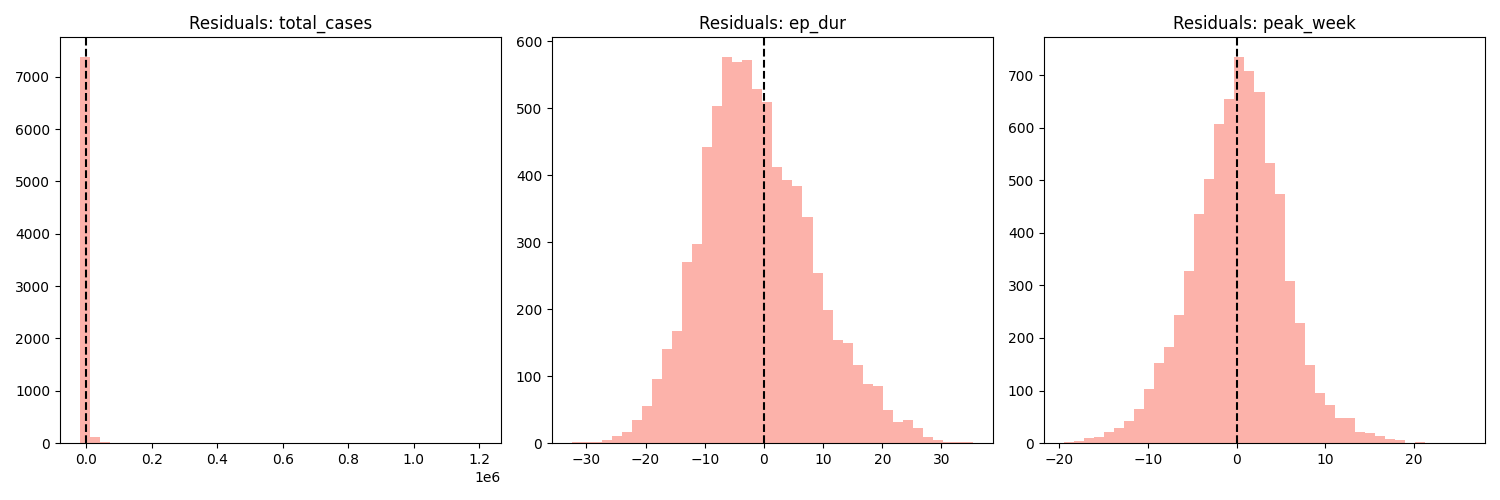
\includegraphics[width=0.95\textwidth]{report_assets/residuals_dist.png}
    \caption{Distributions of forecasting residuals across all targets.}
    \label{fig:residuals}
\end{figure}

\section{Climate Forcing}
Correlations between quarterly climate anomalies and epidemic outcomes (Figure \ref{fig:climate}) elucidate the environmental drivers prioritized by the model.

\begin{figure}[H]
    \centering
    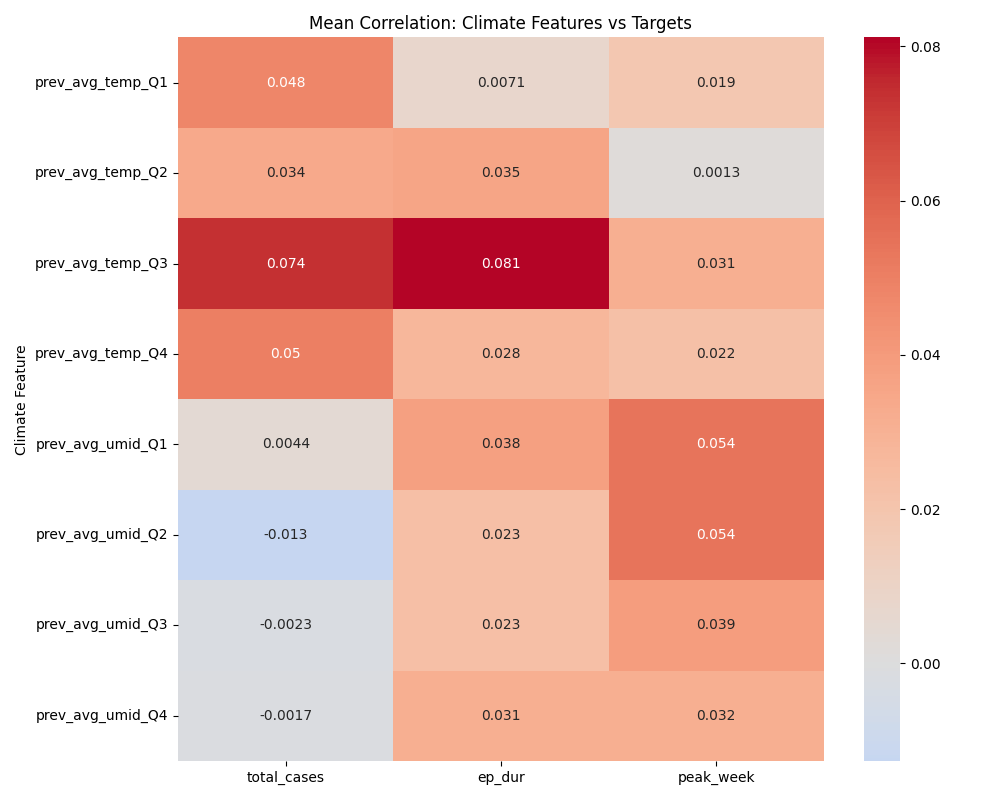
\includegraphics[width=0.8\textwidth]{report_assets/climate_correlations.png}
    \caption{Correlation matrix between quarterly climate metrics and epidemic outcomes.}
    \label{fig:climate}
\end{figure}

\section{Feature Importance}
Variable importance analysis (Figure \ref{fig:importance}) confirms that while lagged epidemiological metrics are primary drivers, climate and population features contribute significantly to non-linear dynamics.

\begin{figure}[H]
    \centering
    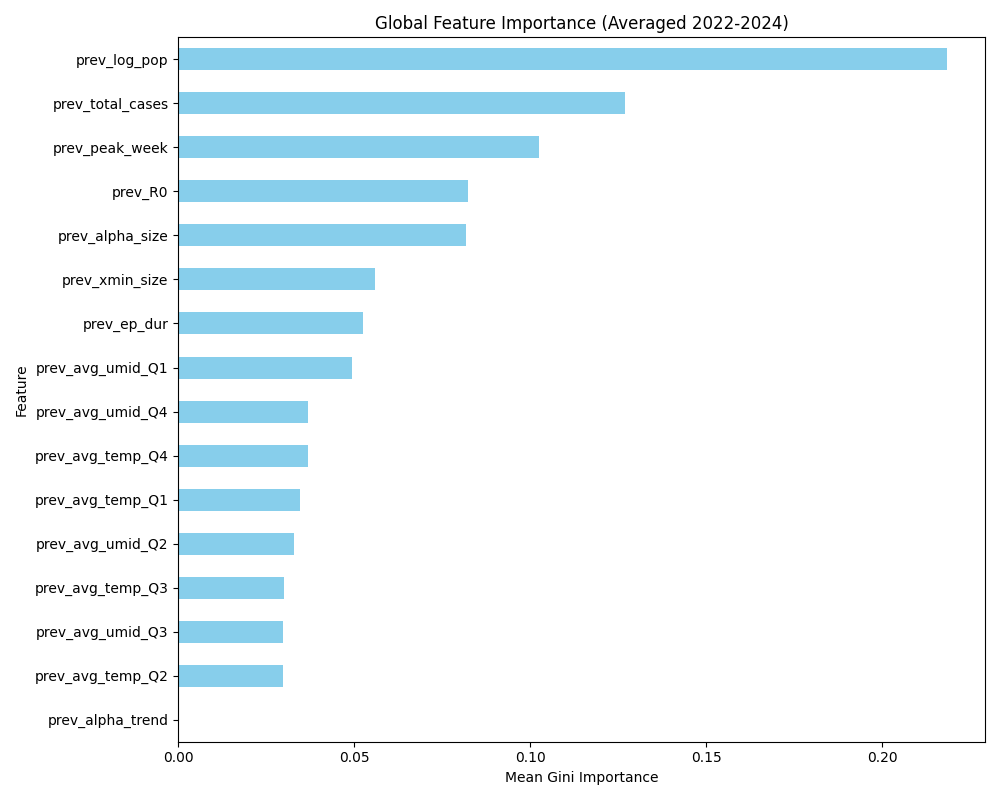
\includegraphics[width=0.85\textwidth]{report_assets/global_importance.png}
    \caption{Global Variable Importance (Averaged 2022-2024).}
    \label{fig:importance}
\end{figure}

\chapter{Conclusion}
The exhaustive analysis demonstrates that for the recent cycles, \textbf{PE} achieved the highest predictive performance. The integration of structural (Power Law), environmental (Climate), and demographic (Population) features creates a robust framework capable of explaining a significant portion of the variance in Dengue outbreaks across heterogeneous Brazilian territories.

\end{document}
